\chapter{Introducción}
\label{chap:introduccion}


\section{Los Desechos Espaciales}


{\bf{Definici\'on:}}{\it{ Son Desechos Espaciales todos los objetos construidos por el hombre, incluyendo fragmentos o partes de los mismos, que orbtian la Tierra o reingresan a la atm\'osfera y no son funcionales, es decir, han perdido su capacidad operativa.}} \cite{iadcguide}\\

En la actualidad se contabilizan m\'as de 16000 objetos catalogados que orbitan la tierra. Las tecnolog\'ias actuales de rastreo permiten identificar y determinar trayectorias para objetos de tamaños mayores a 10 cent\'imetros situados en \'orbitas bajas (LEO), y mayores a 1 metro en \'orbitas geoestacionarias (GEO). Los mismos se rastrean, utilizando t\'ecnicas de radar e instrumentos \'opticos respectivamente.\\

Distintos modelos y an\'alisis muestran que la distribuci\'on de los sat\'elites y desechos que orbitan la Tierra no es homog\'enea. La relaci\'on entre la densidad de objetos y la altura a la que se encuentran, señala que existen regiones m\'as comprometidas, donde la probabilidad de colisi\'on es mayor.\\

En particular, las \'orbitas LEO con un rango de alturas entre los 600 y los 1000 kil\'ometros, son las m\'as superpobladas debido a su utilidad para la observaci\'on de la Tierra y contienen casi el 70 \% de todos los objetos catalogados. Ver Figura \ref{fig:Dvsaltura}

\begin{figure}[!h]
  \centering
  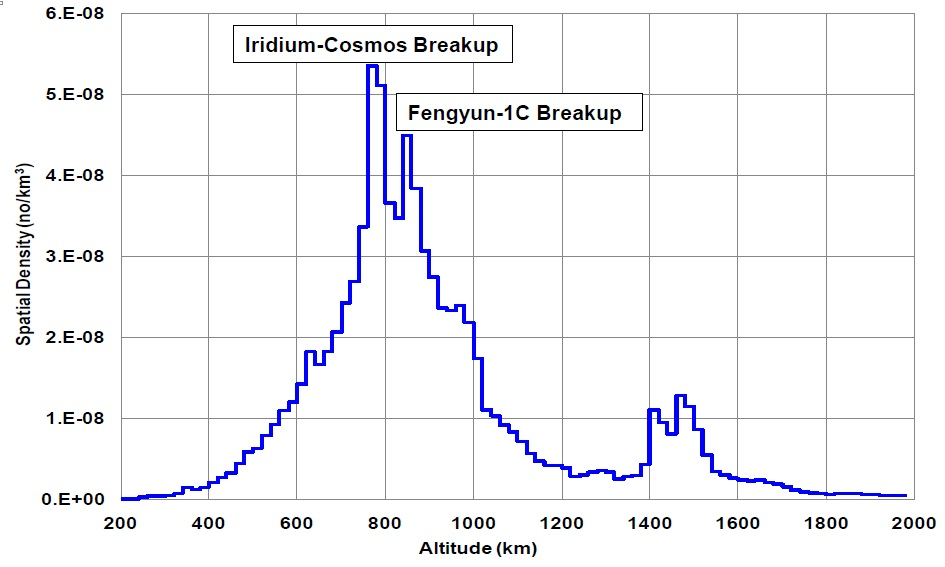
\includegraphics[width=0.9\textwidth]{imagenes/SDvsaltura2011}
  \caption[Distribuci\'on de Desechos seg\'un la altura en \'orbitas LEO]{Densidad de Objetos seg\'un la altura}
  \label{fig:Dvsaltura}
\end{figure}

En alturas menores a los 500 km aproximadamente, el efecto de frenado atmosf\'erico, influye sobre los objetos, disminuyendo su altura hasta {\bf{dar numero preciso}} finalmente se desintegran o caen a la superficie. No obstante este efecto decrece significativamente cuando aumenta la altura, y superados los 500 kil\'ometros el efecto es casi despreciable y los objetos pueden habitar la regi\'on por decenas de a\~nos, en forma no funcional, si no se preveen operaciones expl\'icitas para provocar el re-ingreso.\\ 

Ya hace algunos a\~nos {\bf{dos decadas¡?}}la comunidad espacial investiga la problem\'atica y las consecuencias de la generaci\'on de desechos espaciales. Entre los distintos panoramas, uno que ha despertado particular atenci\'on, es el estudio de las m\'ultiples colisiones.\\
En 1978  estudios predictivos hechos por D. Kessler y Cour-Palais\\
 \cite{kessler0}, anunciaban el riesgo del efecto en cascada que podr\'ian producir las colisiones, aumentando los desechos en un camino catastr\'ofico sin fin y mostrando que los desechos generados por colisiones superar\'ian los impactos por meteoritos.\\

\section{El Riesgo de Colisi\'on}
{\bf{sumar proyectos actuales worldweb \& space X}}
Seg\'un un informe de la \ac{ESA} desde el origen de la era espacial, con el sat\'elite ruso Sputnik en 1957, hasta la actualidad, m\'as de 4900 lanzamientos han puesto en \'orbita del orden de 6600 sat\'elites, de los cuales unos 3600 permanecen en el espacio y s\'olo un peque\~no porcentaje {\bf{7\%}}, correpondiente a 1000, cumplen funciones todav\'ia.\\
Con la tasa actual de 60 a 70 lanzamientos de nuevos sat\'elites por a\~no, sumado a las rupturas que, seg\'un tasas hist\'oricas, ocurren a un promedio de 4 o 5 por a\~no, el n\'umero de desechos aumentar\'a en forma continua. Como consecuencia directa, la probabilidad de colisiones aumenta en una relaci\'on cuatro veces mayor \cite{esaSD}.\\

Un an\'alisis completo del Riesgo de Colisi\'on, abarca: (esquematizar)

\begin{itemize}
\item Identificar las situaciones de encuentro.
\item Analizar la situaci\'on del encuentro.
\item Ejecutar maniobras de mitigaci\'on del riesgo si fuera necesario.
\item Iterar el proceso con minuciocidad para no ofrecer soluciones moment\'aneas que generen nuevos riesgos de colisi\'on.
\end{itemize}

\subsection*{Identificaci\'on de las situaciones de encuentros:}
A partir de los datos generados por las redes de rastreo, se propagan las trayectorias orbitales y, bajo ciertos criterios definidos previamente, se detectan los acercamientos no deseados. En esta idea subyace la definici\'on de {\it{Encuentro}}.\\
Son pocos los organismos y agencias capaces de realizar este procedimiento, incorporando a sus predicciones todos los objetos catalogados y/o rastreados.\\
En un formato m\'as simplificado, el inter\'es se enfoca en una misi\'on en particular y se desarrollan filtros, para procesar encuentros analizando una menor cantidad de objetos.\\


\subsection*{An\'alisis de la situaci\'on del encuentro: }
El mismo consiste en estudiar el panorama con mayor profundidad y detalle, sumando informaci\'on m\'as confiable en la determinaci\'on orbital, y calculando par\'armetros estad\'isticos, como la Probabilidad de Colisi\'on (PoC).\\
A medida que se aproxima la fecha en la que se predice el encuentro, se tiene mejor conocimiento de la \'orbita de los objetos involucrados, pero menor tiempo de reacci\'on en la toma de decisiones. Es decir, en el an\'alisis del encuentro se busca un balance entre los tiempos que conlleve el estudio para alcanzar la confiabilidad necesaria, y el margen que se requiere para, por ejemplo, planificar una maniobra.\\
En este item en particular se enfoca este trabajo.\\

Metodolog\'ia Akella \& Alfriend.\\

\subsection*{realizaci\'on de una maniobra}
Si la situaci\'on lo ameritara, la \'unica manera de evitar una colisi\'on es la {\bf{realizaci\'on de una maniobra}}, conocidas como Maniobras de Mitigaci\'on de Riesgo (RMM). No obstante, modificar la trayectoria de un objeto, siempre presupone una evaluaci\'on a priori de que no vaya a producirse una colisi\'on. De manera, que en este punto, se vuelve al item inicial y se repite el proceso iterativamente.\\ 



La primera colisi\'on catastr\'ofica que se registra, ocurri\'o entre el sat\'elite ruso KOSMOS \- 2251 que hab\'ia quedado fuera de servicio y el sat\'elite operativo IRIDUM33 de la constelaci\'on de IRIDIUM en el a\~no 2009.\\
El evento marc\'o la materializaci\'on de una situaci\'on que se preve\'ia que pod\'ia ocurrir y ofici\'o de catalizador de los estudios vinculados a la predicci\'on, an\'alisis y mitigaci\'on del riesgo de colisi\'on.\\
La exitosa Misi\'on SAC-D/AQUARIUS de la CONAE en convenio con la \ac{NASA}, contabiliz\'o del orden de cinco RMM registradas, a lo largo de su vida \'util [10]. Mientras que la \ac{ISS} realiza casi una maniobra de riesgo de colisi\'on por año, dada su envergadura.\\
CONCEPTO DE MIDDLE MAN.\\
CONCEPTO DE COLLABORATIVE WORK ENVIRONMENT. (close loop process)

Con el creciente avance de la tecnolog\'ia y el acceso al espacio, aumenta la poblaci\'on de objetos que orbitan la Tierra, ya sean  misiones operativas o desechos espaciales. Con esta perspectiva, varios estudios alertan que las colisiones en \'orbita podr\'ian convertirse en las principales fuentes de generaci\'on de nuevos desechos espaciales. \cite{KlinkradChapter8}\\

\section{Las Regulaciones Nacionales e Internacionales}

Dado el car\'acter global de esta problem\'atica, distintas naciones y agencias internacionales con gran desarrollo y actividad espacial, se han estado organizado en la b\'usqueda de acuerdos y buenas pr\'acticas. Entre los organismos que coordinan las recomendaciones, se encuentran:\\

\begin{itemize}
\item {\small{COPUOS: Committee of the Peacefull Uses of Outer Space (ONU)}}
\item {\small{IADC: Inter-Agency Space Debris Coordination Committee}}
\item {\small{CCSDS: Consultative Committee for Space Data Systems}}
\end{itemize}

As\'i mismo, en lo que respecta a los l\'imites de este trabajo, podemos citar las siguientes Normas, Recomendaciones y Legislaci\'on:\\

\begin{itemize}
\item {\small{Convenio sobre Responsabilidad Internacional por da\~nos causados por objetos espaciales. ONU - (29-03-72)}}
\item {\small{Ley 23.335 (19-08-86) - Arg. Suscribe al Convenio de ONU.}}
\item {\small{Space Debris Mitigation Guidelines - IADC}}
\item {\small{ISO 24113:2011 {\it{Space Debris mitigation requirements}}}}
\item {\small{ISO/TR 16158:2013 {\it{Space Systems - Avoiding collision with orbiting objects}}}}
\item {\small{ISO 19389:2014 {\it{Space data and information transfer Systems}}}}

\end{itemize}

\section{Antecedentes}
En este contexto, ya existen claros antecedentes que abordan la problem\'atica con sus respectivos soportes inform\'aticos. (ver tabla \ref{tab:sisal})
\begin{table}[!h]
\centering
\begin{tabular}{|l|p{5cm}|p{6cm}|}
\hline
Herramienta & Desecripci\'on & Proveedor/Agencia\\
\hline
{\bf{CARA}} & {\it{Conjunction Assessment Risk Analysis}} & NASA Robotic Conjunction Assessment Risk Analysis group, en convenio con la empresa a.i. solutions, Inc.\\
\hline
{\bf{SOCRATES}} & {\it{Satellite Orbital Conjuction Reports Assessing Threatening Encounters in Space}}, servicio web v\'ia Celestrack.com & CSSI (Center for Space Standards \& Innovation) de la agencia AGI: Analytical Graphics, Inc.\\
\hline
{\bf{CRASS}} & {\it{Collision Risk Assessment tool}} & Desarrollado por la
empresa GMV, que presta servicios al Centro Europeo de Operaciones
Espaciales (ESOC) - Darmstadt, Alemania. \cite{alarconRodriguez}\\
\hline
{\bf{CAESAR}} & {\it{Conjuction Analysis and Evaluation Service, Alerts and Recommendations}} & Agencia francesa CNES, que utiliza como soporte el Software JAC {\it{Java for Assessment of Conjunctions}}.\cite{laporte}\\
%\hline
%closeap - ant\'on & & ESA\\
\hline
{\bf{CRAMS}} & {\it{Collision Risk Assessment and Mitigation System}} & Canadian Space Agency (CSA). \cite{babiker}\\
\hline
\end{tabular}
\caption[Sistemas de Alerta]{Sistemas de Alertas de distintas Naciones y Agencias}
\label{tab:sisal}
\end{table}

\section{La Unidad de Desechos Espaciales de la CONAE}
De acuerdo con el Plan Nacional Espacial: {\bf{ Argentina en el Espacio 2004-2015}} [5], las misiones de la CONAE, fundamentalmente pensadas para observaci\'on de la Tierra, ocupan \'orbitas bajas de dise\~no estrat\'egico. Es decir, se ubican en regiones de mucha demanda y en consecuencia se encuentran expuestas a un alto riesgo de colisi\'on.\\
En nuestro pa\'is, compete a la Unidad de Desechos Espaciales de la Secretaria General de la CONAE; quien tiene la facultad de mantener las relaciones con los organismos internacionales, garantizar que se cumplan los distintos convenios y acuerdos a los que Argentina ha adherido, como por ejemplo el {\it{Convenio sobre la Responsabilidad Internacional por da\~nos causados por objetos espaciales}}, suscripto por la Rep\'ublica Argentina el 29 de marzo de 1972. (LEY N 23.335, sancionada: Julio 30 de 1986 - promulgada: Agosto 19 de 1986.1).\\
 As\'i mismo, como miembro parte de la ONU (Organizaci\'on de las Naciones Unidas), responde ante el \ac{COPUOS} en temas como {\bf{mejorar esta frase}} el estudio y mitigaci\'on del ambiente de desechos espaciales.\\

En la actualidad, las \'unicas naciones que cuentan con una red de rastreo con capacidad de detectar, rastrear y catalogar objetos son EE.UU y Rusia. De manera que Argentina planifica y ejecuta sus RMM a partir de informaci\'on que le proveen servicios externos.\\

El an\'alisis de posible colisi\'on, es uno de los temas que se abordan con mayor delicadeza dentro del \'area espacial y dado el nivel de riesgo que implica, la CONAE contrata un servicio de asesoramiento y control para la planificaci\'on de las operaciones vinculadas al alerta por colisi\'on.\\
Ofrecer un servicio que reemplace al que utiliza actualmente en CONAE, es impensado y escapa por mucho a los alcances de este trabajo. No obstante, hemos desarrollado una herramienta que permite una clara caracterizaci\'on de la situaci\'on y un mayor conocimiento en el di\'alogo e intercambio de informaci\'on con los organismos y agencias que proveen el servicio y asesoramiento. As\'i mismo, se piensa como un planteo preliminar, con versatilidad para ser testeado, perfeccionado y ampliado a largo plazo.\\

\section{Planteo del Problema}

Llega un CDM que anuncia un riesgo de colisi\'on en el tiempo futuro $t_{ca}$, ¿qu\'e cosas me pregunto?

Preguntas:\\

\begin{enumerate}
 \item ¿Por qu\'e hablamos de probabilidad?
 \item ¿Con qu\'e error conozco la posici\'on de la Misi\'on para la \'epoca actual?\\
 \item ¿Con qu\'e error conozco la posici\'on del desecho para la \'epoca actual?\\
 \item ¿Con qu\'e error conozco la posici\'on de la Misi\'on para la \'epoca $t_{ca}$?\\
 \item ¿Con qu\'e error conozco la posici\'on del desecho para la \'epoca $t_{ca}$?\\
\end{enumerate}

\begin{enumerate}
 \item Error de la Misi\'on en la \'epoca actual: La posici\'on y velocidad se plasma en los productos que genera el CODS, a trav\'es de sus efem\'erides predichas y o precisas. El error asociado ... {\textcolor{red}{¿? : documento CODS y/o dato CDM}} - {\textcolor{red}{En nuestro trabajo utilizamos TLEs para su estimaci\'on y la generaci\'on de la matriz de covarianza.}} Como mostraremos m\'as adelante en el capítulo \ref{chap:metodologia}...\\
 \item Error del Desecho en la \'epoca actual: {\textcolor{red}{¿?:dato CDM}} - M\'etodo de Osweiler. Funci\'on de Ajuste a partir de la tendencia. (Validaci\'on utilizando datos CODS para comparar los resultados de la funci\'on de ajuste) - JSPoC no cuenta con info de maniobras planificadas.
 
\end{enumerate}





\section{Objetivos}

La herramienta ARxCODE para el An\'alisis de Riesgo por Colisi\'on con Desechos, que presentamos en esta tesis, consiste en un software que ser\'a montado sobre la estructura actual con la que cuenta el departamento de Din\'amica Orbital, y ser\'a utilizado por operadores del sector con amplios conocimientos del area.\\
\begin{figure}[!h]
\centering
  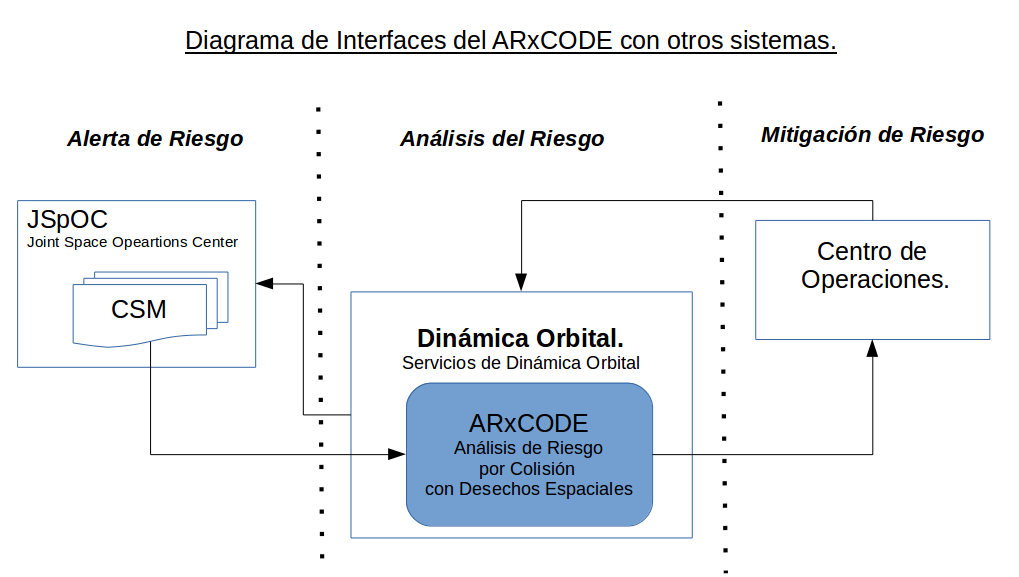
\includegraphics[width=0.7\textwidth]{imagenes/interfasessistemas}
\end{figure}
{\bf{Revisar este esquema para que cierre y vuelva a JSPoC}}
El mismo oficiar\'a de intermediario entre los organismos internacionales que proveen los mensajes de alerta (CDM) y el operador de din\'amica orbital, quien se encargar\'a de procesar la informaci\'on con las facilidades que ARxCODE provee y generar los reportes necesarios para el intercambio de informaci\'on y la toma de decisiones.\\ 

